
\medskip

\parbox{0.66\linewidth}{Le \og hand-spinner \fg{} est une sorte de toupie plate qui tourne sur elle-même.

On donne au \og hand-spinner \fg{} une vitesse de rotation initiale au temps $t = 0$, puis, au cours du temps, sa vitesse de rotation diminue jusqu'à l'arrêt complet du \og hand-spinner \fg{}.

Sa vitesse de rotation est alors égale à $0$.

Grâce à un appareil de mesure, on a relevé la vitesse de rotation exprimée en
nombre de tours par seconde.}\hfill
\parbox{0.32\linewidth}{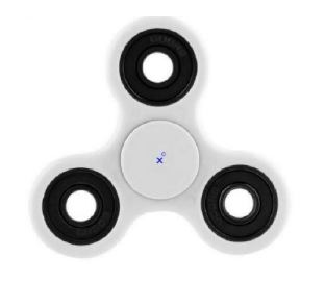
\includegraphics[width=2.6cm]{handspinner}}

\medskip

Sur le graphique ci-dessous, on a représenté cette vitesse en fonction du temps exprimé en seconde :

\begin{center}
\psset{xunit=0.1cm,yunit=0.4cm}
\begin{pspicture}(-20,-1)(100,25)
\rput{90}(-8,12.5){\footnotesize Vitesse de rotation (en nombre de tours par seconde) }
\uput[d](50,-1){\footnotesize Temps (en s)}
\multido{\n=0+4}{26}{\psline[linewidth=0.2pt](\n,0)(\n,25)}
\multido{\n=0+1}{26}{\psline[linewidth=0.2pt](0,\n)(100,\n)}
\psaxes[linewidth=1.25pt,Dx=20,Dy=5,labelFontSize=\scriptstyle](0,0)(0,0)(100,25)
\psline[linewidth=1.5pt](0,20)(94,0)
\end{pspicture}
\end{center}
\begin{flushright}
\emph{\tiny Inspiré de: https://www.sciencesetavenir.frlfondamental/combien-de-temps-peut-tourner-votre-hand-spinner-112808}
\end{flushright}

\medskip

\begin{enumerate}
\item Le temps et la vitesse de rotation du \og hand-spinner \fg{} sont-ils proportionnels? Justifier.
\item Par \textbf{lecture graphique}, répondre aux questions suivantes:
	\begin{enumerate}
		\item Quelle est la vitesse de rotation initiale du \og hand-spinner \fg{} (en nombre de tours par seconde) ?
		\item Quelle est la vitesse de rotation du \og hand-spinner \fg{} (en nombre de tours par seconde) au bout d'une minute et vingt secondes ?
		\item Au bout de combien de temps, le \og hand-spinner \fg{} va-t-il s'arrêter ?
	\end{enumerate}
\item  Pour calculer la vitesse de rotation du \og hand-spinner \fg{} en fonction du temps $t$, notée $V(t)$, on utilise la fonction suivante :
	
\[V(t) = - 0,214 \times t + V_{\text{initiale}}.\]
	
$\bullet~~$ $t$ est le temps (exprimé en s) qui s'est écoulé depuis le début de rotation du \og hand-spinner \fg{} ;
	
$\bullet~~$ $V_{\text{initiale}}$ est la vitesse de rotation à laquelle on a lancé le \og hand-spinner \fg{} au départ.
	\begin{enumerate}
		\item On lance le \og hand-spinner \fg{} à une vitesse initiale de $20$ tours par seconde. Sa vitesse de rotation est donc donnée par la formule : 
		
		\[V(t) = - 0,214 \times t + 20.\]
		
Calculer sa vitesse de rotation au bout de $30$~s.
		\item Au bout de combien de temps le hand-spinner va-t-il s'arrêter ? Justifier par un calcul.
		\item Est-il vrai que, d'une manière générale, si l'on fait tourner le hand-spinner deux fois plus vite au départ, il tournera deux fois plus longtemps ? Justifier.
	\end{enumerate}
 \end{enumerate}


